% !TEX root = ../main.tex

\section{Related Work}
\label{sec:org2aceb9f}

% Beyond identifying object types (see YOLO~\cite{YOLO} and its successors),
% performing face recognition (see FaceNet\cite{FaceNet} and its successors) on
% segments of an image, n
% Neural networks are increasingly becoming better at predicting more abstract
% concepts via deeper networks, representation learning and
% self-supervision~\citep[see, e.g.,][]{SS,Rep}. There is a significant volume
% of recent work on building neural networks with a high-level of abstract
% understanding in the embedding space~\mdr{REF}. However, research on
% developing optimization frameworks that are adapted for these abstract
% concepts in the output space is limited. In the next sections we detail
% some of this related work and discuss it relation to the research in this paper.

Existing algorithmic solutions to deal with FIMPUL tasks can be divided into
\emph{fit-data-to-algorithm} solutions, which map FIMPUL problems to a known
problem formulation like multi-class uni-label classification, and
\emph{fit-algorithm-to-data} solutions, which adapt existing classification
algorithms for the problem at hand~\citep{multilabelMethods}.

\subsection{Fit-data-to-algorithm}
Commonly, in fit-data-to-algorithm solutions, cross-entropy losses are used at
training time and thresholding is done at inference time to determine how many
labels should be assigned to an instance.

The \textit{label powerset} approach considers each unique set of labels as
one class in the transformed setting~\cite{multilabelComparison} (e.g. an
instance labeled \textit{Thriller} and \textit{Action}, results in the
creation of the class \textit{Thriller and action}). Alternatively,
\textit{ranking by pairwise comparison} is a solution where the dataset is
duplicated for each possible label pairs. Each duplicated dataset has
therefore two classes and only contains instances that have at least one of
the labels in the label pair. Different ranking methods
exist~\cite{pairwiseBinary, pairwiseNet}.

More recently, hierarchical datasets such as
DBpedia\footnote{\url{https://wiki.dbpedia.org/develop/datasets/latest-core-dataset-releases}}
are often used to finetune BERT-based models~\cite{XLNet, bigBird}. In both
publications, cross-entropy is used to predict the labels.

\subsection{Fit-algorithm-to-data}
Conversely, in the fit-algorithm-to-data solutions, elements of the learning
algorithm are changed (such as the back propagation procedure or the task).

Early representatives of fit-algorithm-to-data stem from heterogenous domains
of machine learning. Multi-Label k-Nearest Neighbors \cite{ML-KNN},
Multi-Label Decision Tree \cite{ML-DT}, Ranking Support Vector Machine
\cite{multilabelSVM} and Backpropagation for Multi-Label Learning
\cite{multilabelBackprop}. More recently, two papers introduced the idea of
multitask learning for \emph{label prediction} and \emph{label count
prediction} for text (ML\(_{\text{NET}}\)) \cite{multitaskLabel} and image
\cite{multitaskLabelImages, tencent} data. The latter research is loosely
catered towards object detection (although not formally presented as such) and
is thus out-of-scope: elements in a picture are predicted that tend to be
unilabel as defined by the groundtruth (e.g. cat, flower, vase, person, bottle
etc.).

An important shortcoming shared by both \emph{fit-data-to-algorithm} and
\emph{fit-algorithm-to-data} is the lack of a holistic approach for both label
count and label prediction.

\begin{figure*}[t!]
\centering
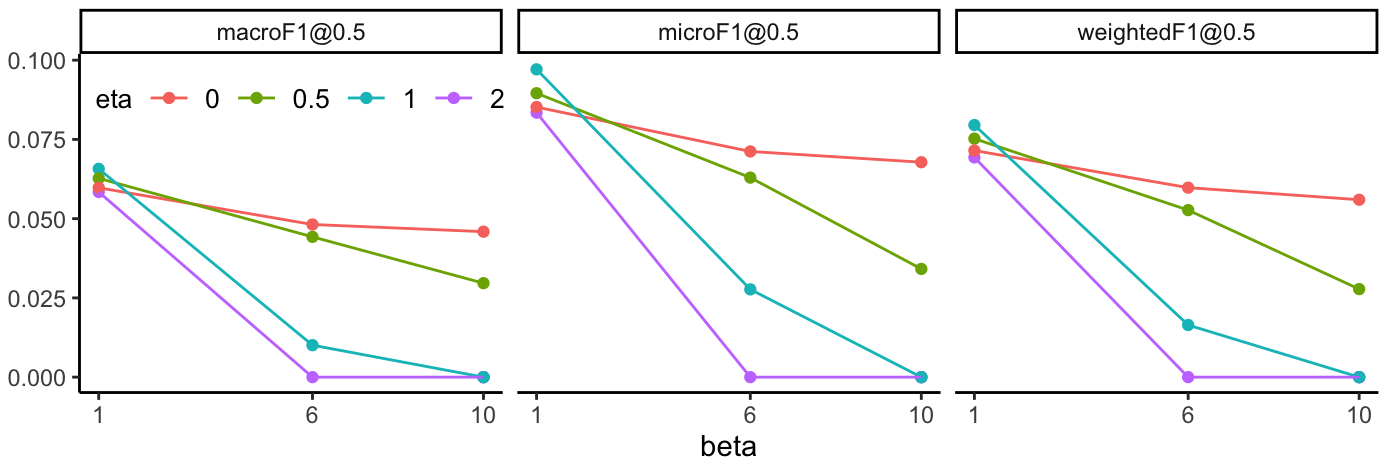
\includegraphics[width=.9\linewidth]{./images/betaEtaResized.png}
\caption{\label{fig:betaEta}
DistilBert (NLP) + classification head on arXiv2020 – different scores at a 0.5 threshold for different values of $\eta$ and $\beta$ in a sampling region.}
\end{figure*}

\subsection{Thresholding}
\label{subsec:thresh}

Machine learning prediction tasks' output are probabilistic (or a reversible
transformation of a probabilistic measure such as a sigmoid or a soft max
function). At training time, these probabilistic values are compared to binary
values in the case of binary encoding of classes. At inference time, if the
number $n_i$ of labels to be predicted per example is known a priori, it is
natural to assign the $top_{n_i}$ predictions to that
example~\cite{lossTopKError, topKmulticlassSVM}. If the number of labels per
example is unknown a priori, the question remains at inference time as to how
to extract information about the number of labels to assign to each example,
aside from the propensity of labels to be assigned. This is generally done via
a \emph{decision threshold}, that can be set globally for all examples. This
threshold can optimize for specificity or
sensitivity~\cite{decisionThreshold}. In our method, this threshold is
implicitly defined, thanks to the use of metrics that already penalize for
wrong label counts.

Thresholding across classes or examples can be an issue as soon as the number
of labels to predict is unknown. Certain variants of cross-entropy loss
accommodate imbalanced label data  \cite{focalLoss}, but remain agnostic
towards the number of labels to predict. Solutions have been tailored to that
end, starting with determining an ideal global \emph{threshold} depending on
use-cases \cite{threshForF1}, or per-class-thresholding after training
\cite{moviePosters} and eventually abstracting the threshold away via a
\emph{soft-F1} measure \cite{softF1}. In the latter two cases, the task is to
predict genre from movie posters.

\subsection{Metrics as Losses}

Learning to Rank (the practice of using Machine Learning to sort documents
according to their relevance) lead to the widespread use of certain
metrics~\cite{LTR}. In a number of retrieval tasks, a model's out of sample
accuracy is measured on metrics such as AUROC, F1 score, etc. These reflect an
objective catered towards evaluating the model over an entire ranking. Due to
the lack of differentiability, these metrics cannot be directly used as loss
functions at training time (in-sample). A seminal
study~\cite{optimizableLosses} proposed a general framework for deriving
decomposable surrogates from some of these metrics. In our research, we
instead propose decomposable surrogates of the classical confusion matrix
metrics and in particular sigmoidF1, tailored to the problem at hand.

Often, machine learning post-training evaluation metrics (e.g. AUROC, F1) are
not differentiable. If they were decomposable, one could
optimize a model directly on a metric at training time. A general framework
for AUC, AUROC and F1 is presented in \cite{optimizableLosses}, but the
proposed F1 surrogate is not explicitly created for stochastic gradient
descent. Recently, a similar work has been proposed to train a Convolutional
Neural Network (CNN) from scratch with a few millions of images and hundreds
of labels specifically for multilabel tasks \cite{tencent}. This task is
loosely related to object detection, similarly to \cite{multitaskLabelImages}
mentioned in the previous paragraph.

% The proposed method is positioned in the lineage of \emph{algorithm
% adaptation}, using \emph{metric as losses} and allowing for dynamic
% \emph{thresholding}.

% This section will be guided by the previous section's formulation of the multitags problem, we will therefore focus on \emph{fit-algorithm-to-data}, \emph{metrics as losses} and \emph{thresholding}.

% \subsection{fit-algorithm-to-data}
% \label{sec:org150a474}

% % Early representatives of \emph{fit-algorithm-to-data} stem from heterogenous domains of machine learning. Multi-Label k-Nearest Neighbors \cite{ML-KNN}, Multi-Label Decision Tree \cite{ML-DT}, Ranking Support Vector Machine \cite{multilabelSVM} and Backpropagation for Multi-Label Learning \cite{multilabelBackprop}. More recently, two papers introduced the idea of multitask learning for \emph{label prediction} and \emph{label count prediction} for text (ML\(_{\text{NET}}\)) \cite{multitaskLabel} and image \cite{multitaskLabelImages} data. The latter research is loosely catered towards object detection (although not formally presented as such) and is thus out-of-scope: elements in a picture are predicted that tend to be unilabel as defined by the groundtruth (e.g. cat, flower, vase, person, bottle etc.).

% \subsection{Metrics as losses}
% \label{sec:orgb0a9d21}

% Often, machine learning post-training evaluation metrics (e.g. AUROC, F1) are not differentiable. There are motivations \todo{which motivations} for optimizing a model directly on a metric at training time. A general framework for AUC, AUROC and F1 is presented in \cite{optimizableLosses}, but the proposed F1 surrogate remains short of being explicitly derived for stochastic gradient descent. \todo{check again with the authors if I can't get inspired from their work}. Recently, a similar work has been proposed to train a Convolutional Neural Network (CNN) from scratch with a few millions of images and hundreds of labels specifically for multilabel tasks \cite{tencent}. This task is loosely related to object detection, similarly to \cite{multitaskLabelImages} mentioned in the previous paragraph.


% in reformulating loss functions to accomodate sparsity in the data, to optimize directly for the metric at hand or to do thresholding posthoc (see movie posters).

% \subsection{Thresholding}
% \label{sec:org8295f09}

% \emph{thresholding} accross classes or examples can be an issue as soon as the number of labels to predict is unknown. Certain variants of cross-entropy loss accommodate imbalanced label data  \cite{focalLoss}, but remain agnostic towards the number of labels to predict. Solutions have been tailored to that end, starting with determining an ideal global \emph{threshold} depending on use-cases \cite{threshForF1}, or per-class-thresholding after training \cite{moviePosters} and eventually abstracting the threshold away via a \emph{soft-F1} measure \cite{softF1} \todo{say more about this method}. In the latter two cases, the task is to predict genre from movie posters.



% The proposed method is positioned in the lineage of \emph{fit-algorithm-to-data}, using \emph{metric as losses} and allowing for dynamic \emph{thresholding}.

% \todo{compare to this:} \cite{lossComp}

% \todo{Hamming Loss}
% % \todo{Precision@K, Recall@K, NDCG@K}
% \todo{MLTSVM loss and the three-way loss inspired by it} \cite{MLTSVM} and \cite{MLTSVMThreeway}

% We propose a dynamic thresholding mechanism auto-tuned at training time.


% ** weak labels
% (unsure the labels are correct)

% - https://people.cs.pitt.edu/~kovashka/ye_zhang_kovashka_iccv2019_cap2det.pdf


% ** implementations

% *** movies

%  [[https://www.analyticsvidhya.com/blog/2019/04/build-first-multi-label-image-classification-model-python/][movie posters with classes]].

%  They have movie titles in them

% *** pretrained resnet on multilabel

%  https://github.com/Tencent/tencent-ml-images

% What happens when using a Resnet pretrained on multilabels

% *** soft F1 score loss

%  https://github.com/ashrefm/multi-label-soft-f1

% https://www.analyticsvidhya.com/blog/2019/04/build-first-multi-label-image-classification-model-python/



% /Optimizing directly for macro F1: By introducing the macro soft-F1 loss, we could train the model to directly increase the metric we care about: the macro F1-score @ threshold 0.5. We could clearly observe the alignment during training and evaluation on successive epochs. When using this loss, we do not have to tune the decision threshold any more. Imagine a multi-label classification system with hundreds of labels, how unstable the system will be if we have to continuously update the optimal threshold for each label. The macro soft-F1 loss comes to the rescue. By using it, we can keep all thresholds fixed at 0.5 and still get an optimal performance from the training process./



%%% Local Variables:
%%% mode: latex
%%% TeX-master: "../main"
%%% End:
